%% Paper 2 -- Journal of Process Control (elsarticle).
%% Compile: latexmk -pdf main.tex   (Overleaf: elsarticle is preinstalled).
%% Figures expected in ../figures/ ; bibliography references.bib in this folder.
\documentclass[review,times]{elsarticle}

\usepackage{amsmath,amssymb}
\usepackage{graphicx}
\usepackage{booktabs}
\usepackage[hidelinks]{hyperref}
\usepackage{url}
\graphicspath{{../figures/}}

\journal{Journal of Process Control}

\begin{document}

\begin{frontmatter}

\title{The conformal selection effect in real-time optimisation: why marginally valid
back-offs over-violate and conditional calibration restores safety}

\author{Bien Busico}
\affiliation{organization={Affiliation to be completed},
             country={Philippines}}

\begin{abstract}
Real-time optimisation (RTO) drives a process toward a quality constraint it cannot
measure online, so it must subtract a back-off, a safety margin, from the specification.
Conformal prediction is the natural distribution-free way to size that back-off from
data. We show that it is unsafe under optimisation. An RTO that optimises against a
marginally valid conformal back-off, even a locally adaptive one, behaves as a selection
mechanism: it drives the operating point to where the margin under-covers the conditional
constraint quantile, and on a rigorous Peng--Robinson distillation twin the realised
violation rate reaches roughly five times the nominal level across the disturbance range.
We identify this conformal selection effect as the optimisation-induced loss of marginal
coverage, and we verify against an oracle, which uses the true conditional quantile, that
the failure lies in the back-off rather than in the chance-constrained formulation.
Restoring safety requires conditional validity. A back-off built from conformalised
quantile regression, combined with an a-posteriori calibration step at the selected
setpoint, returns the realised violation to the oracle level, within a Monte-Carlo band,
at near-oracle profit over the operationally realistic disturbance range. It degrades only
when the disturbance widens several-fold and the conditional estimate runs out of
calibration data, and even then it degrades visibly, through a climbing inflation factor.
A regime map over disturbance magnitude bounds where each back-off controls violation. The
contribution is calibrated safety, not profit: at a well-controlled feed the constraint is
barely active and all methods earn within half a percent of the deterministic optimum. The
mechanism is general, since any conformal interval used as a hard optimisation constraint
is exposed to it, and the portable rule that follows is to size the margin conditionally
and to read the a-posteriori inflation as a signal of data adequacy.
\end{abstract}

\begin{keyword}
real-time optimisation \sep chance-constrained optimisation \sep conformal prediction \sep
conditional coverage \sep constraint back-off \sep distillation
\end{keyword}

\end{frontmatter}

\section{Introduction}
\label{sec:intro}

Real-time optimisation (RTO) recomputes the operating point of a process to maximise an
economic objective as conditions drift. Its value comes from pushing the process against
its constraints; a distillation column earns more as it drives a product composition to
the edge of specification. The constraints that matter most, however, are often on quality
variables that are not measured online. A laboratory assay or an inferential estimate
stands in for a true composition that the controller never sees in real time. To operate
safely against such a constraint, an RTO must subtract a back-off from the specification: a
margin that absorbs the gap between the model's nominal prediction and the realised quality
under an unmeasured disturbance. Sizing that margin is the central difficulty of RTO under
uncertainty. Set it too small and the process violates specification whenever the
disturbance is adverse. Set it too large and the economic benefit of the optimisation is
given away.

Conformal prediction is the natural tool for the job. It turns any predictor into an
interval with a finite-sample, distribution-free coverage guarantee, assuming only that the
data are exchangeable, with no Gaussian residuals and no parametric disturbance law. Taking
the upper edge of a conformal interval as the back-off promises exactly what a chance
constraint asks for, namely coverage of the realised quality at the nominal level, learned
from data, without distributional assumptions. This paper asks whether that promise survives
contact with the optimiser. It does not.

We show that an RTO optimising against a marginally valid conformal back-off is unsafe. A
conformal margin guarantees coverage on average over the calibration distribution of
operating points, but the optimiser does not sample that distribution. It deliberately
seeks the boundary of the feasible region, which is where the margin is tightest relative
to the local risk and therefore where coverage is worst. The argmax is a selection
operator, and it selects for under-coverage. On a rigorous binary-distillation twin
(Figure~\ref{fig:rto}), a back-off that is marginally valid, including a locally adaptive
heteroscedastic one that widens where the data are noisier, yields a realised violation
rate of roughly five times the nominal level across the entire disturbance range. The
failure is structural rather than a consequence of the disturbance being large, and
adaptivity in the width of the margin does not cure it. We call this the conformal
selection effect: the optimisation-induced loss of the marginal coverage guarantee, a
constraint-space analogue of the winner's curse in post-selection inference. The phenomenon
was named in the abstract by the conformal-predictive-programming literature
\citep{zhao2024cpp}, which observed that a decision optimised against sampled constraints is
no longer independent of them. Our contribution is to instantiate it in a process-RTO loop,
to quantify its severity, and to isolate what fixes it.

What fixes it is conditional validity. A back-off built from conformalised quantile
regression \citep{romano2019} targets the conditional constraint quantile at each operating
point rather than a calibration average, so there is no systematic gap between margin and
risk for the optimiser to exploit. The residual finite-sample error is closed by an
a-posteriori calibration at the selected setpoint, in the manner of conformal predictive
programming. On the twin, this conditional method returns the realised violation to the
level of an oracle that knows the true conditional quantile, to within the Monte-Carlo
estimation band, at near-oracle profit over the operationally realistic disturbance range.
The oracle margin, available here because the twin furnishes the plant response, holds the
violation at the nominal level by construction. That it does so confirms that the failure
of the marginal methods lies in the back-off, not in the chance-constrained formulation.

The method is not unconditionally safe, and we map where it holds. Sweeping the disturbance
magnitude produces a regime map. The conditional method tracks the oracle up to roughly
three times the realistic disturbance. A constant margin over-violates and then becomes
infeasible. The a-posteriori inflation factor climbs from near unity to nearly sixfold
before the conditional estimate, too, runs out of calibration data and can no longer
certify the target. That inflation factor is an interpretable diagnostic, since the operator
sees the safety margin being stretched before it breaks. Finally, we are explicit that the
contribution is calibrated safety, not profit. At a well-controlled feed the constraint is
barely active and every method earns within half a percent of the deterministic optimum, so
the value of the conditional method is the violation it removes, not any profit it adds.

The contributions are as follows.
\begin{itemize}
\item \textbf{R1.} We identify and quantify the conformal selection effect in RTO. A
  marginally valid back-off, fixed or locally adaptive, realises roughly five times the
  nominal violation under optimisation, while an oracle conditional margin holds the target.
  This establishes that the failure is the selection effect and not the chance-constraint
  formulation (Sections~\ref{sec:results-selection} and \ref{sec:results-oracle}).
\item \textbf{R2.} We show that conditional validity is the structural remedy. A CQR
  back-off with an a-posteriori calibration step tracks the oracle to within the
  Monte-Carlo band at near-oracle profit over the realistic disturbance range, with the
  a-posteriori inflation reduced from a primary guarantee to a small residual correction
  (Section~\ref{sec:results-fix}).
\item \textbf{R3.} We characterise the disturbance-magnitude regime over which each margin
  controls violation, where a constant margin becomes infeasible, and where the conditional
  method itself is data-starved, reading the a-posteriori inflation as a diagnostic of data
  adequacy (Sections~\ref{sec:results-boundary} and \ref{sec:results-profit}).
\end{itemize}

Section~\ref{sec:related} places the work against RTO under uncertainty, conformal
prediction, and conformal optimisation. Section~\ref{sec:methods} formalises the
chance-constrained RTO, the four back-offs, the selection-effect argument, and the
a-posteriori step. Section~\ref{sec:case} describes the twin and the experimental design,
Section~\ref{sec:results} reports the regime map, and Section~\ref{sec:discussion} draws out
the general design rule, the limitations, and the bridge to a closed-loop extension with an
online soft sensor.

\section{Related work}
\label{sec:related}

This work sits at the meeting point of three lines: real-time optimisation under
uncertainty, conformal prediction and its conditional-validity theory, and the recent use
of conformal prediction inside optimisation. We review each in turn and then state the gap.

\subsection{Real-time optimisation under uncertainty}

The dominant paradigm for steady-state RTO under plant--model mismatch is modifier adaptation
\citep{marchetti2009,chachuat2009}, which adds first-order correction terms to the model cost
and constraints so that, on convergence, the model-based optimum is a KKT point of the plant.
Modifier adaptation corrects the nominal prediction, but it does not by itself supply a
probabilistic margin against an unmeasured disturbance. Safety against violation is handled
implicitly, through conservative tuning or through filtering of the modifiers.

A data-driven branch replaces or augments the modifiers with learned surrogates.
\citet{delrio2021}, extending the Gaussian-process modifier-adaptation line
\citep{delrio2019}, use Gaussian-process regression to capture the cost and constraint
mismatch non-parametrically, and they embed trust-region and acquisition-function ideas from
Bayesian optimisation to manage risk during exploration. There the GP mean corrects the
constraint and the GP variance drives excitation and sizes the trust region. The scheme is
probabilistic in its exploration, yet it does not issue a distribution-free, finite-sample
coverage guarantee on the constraint, and its risk control is trust-region containment rather
than a calibrated back-off. The closely related stochastic-MPC line
\citep{bradford2019,bradford2020} does subtract explicit GP-posterior back-offs from
constraints, but in a receding-horizon control setting and under a Gaussian posterior
assumption.

The classical route to explicit probabilistic constraints is chance-constrained programming
\citep{li2008}, which constrains the probability of satisfaction directly, computes
joint-constraint probabilities by sampling under an assumed, typically multivariate-normal,
disturbance law, and trades feasibility against profitability through the miss level. This is
the formulation we adopt in Eq.~\eqref{eq:chance}. The difference here is that the back-off
enforcing it is built distribution-free from data rather than from an assumed Gaussian law.

\subsection{Conformal prediction and conditional validity}

Conformal prediction \citep{vovk2005,angelopoulos2023} converts any point predictor into a
set with a finite-sample, distribution-free marginal coverage guarantee under
exchangeability. Split conformal and its locally weighted variants \citep{lei2018} rescale
the residual by a spread estimate so that the interval width adapts to the input, and
conformalised quantile regression \citep{romano2019} goes further by conformalising a
quantile-regression estimate so that the interval targets the conditional quantile while
retaining the marginal guarantee. All of these methods deliver coverage on average over the
calibration distribution.

The limit of that guarantee is the subject of a conditional-validity literature. Exact
distribution-free conditional coverage is impossible without further assumptions
\citep{vovk2012,leiwasserman2014}, and recent work characterises and partially restores
conditional guarantees \citep{gibbscherian2023}. A parallel strand relaxes exchangeability
itself, for distribution shift and dependent data
\citep{tibshirani2019,barber2023,gibbs2021}. The gap between marginal and conditional
validity is precisely what an optimiser exploits in this paper, because a margin calibrated
on average under-covers at the specific operating point an optimiser selects.

\subsection{Conformal prediction inside optimisation}

Conformal prediction has recently been brought inside chance-constrained optimisation.
Conformal predictive programming (CPP; \citealt{zhao2024cpp}) uses the conformal quantile
lemma to reformulate a chance-constrained program as a deterministic quantile-constrained
one, supporting any conformal variant and providing feasibility guarantees. Of central
importance for the present work, CPP observes that once a decision is optimised against
sampled constraint evaluations those evaluations are no longer independent of the decision,
so the exchangeability that underwrites the conformal guarantee is broken by the optimisation
itself, and it restores a guarantee a posteriori by recalibrating the selected solution on a
second, independent dataset. Related uses of conformal sets to certify safety in optimisation
and control include online-conformal safety guarantees for Bayesian optimisation
\citep{zhang2024} and conformal back-offs proposed for predictive control.

CPP supplies the a-posteriori calibration machinery this paper uses
(Section~\ref{sec:methods-apost}) and names the loss-of-independence mechanism in the
abstract. What it does not do, and what no work in the RTO literature above does, is
instantiate the mechanism in a process real-time optimisation loop, quantify how severely a
marginally valid, including locally adaptive, back-off is degraded by the optimiser, or
separate the two remedies the problem actually needs: a conditional construction to remove
the systematic selection bias, with a-posteriori calibration left to cover only the
finite-sample residual. CPP treats the a-posteriori step as the primary guarantee. We show
that without conditional validity that step is either large or infeasible, and that a
conditional back-off makes it small.

\subsection{Gap}

No existing treatment does three things together. It does not place a distribution-free
conformal constraint back-off inside a chemical-process RTO loop; it does not expose and
quantify the optimiser-induced selection effect that drives a marginally valid margin to
several times its nominal violation; and it does not identify conditional validity as the
structural remedy, relegating a-posteriori calibration to a residual correction and reading
its inflation factor as a diagnostic of data adequacy. This paper provides that treatment on
a rigorous debutaniser twin, and it maps the disturbance regime over which the treatment
holds. The soft-sensor framework of the companion paper \citep{companion2026} supplies the
model-based estimate of the unmeasured constraint that the back-off corrects; here that
estimate is taken as given and the focus is the back-off itself.

\section{Problem formulation and methods}
\label{sec:methods}

\subsection{Chance-constrained real-time optimisation under an unmeasured disturbance}
\label{sec:methods-rto}

We consider steady-state real-time optimisation of a distillation column whose
product-quality constraint cannot be measured online (Figure~\ref{fig:rto}). The decision is
the operating point $u=(R,D)$, with $R$ the reflux ratio and $D$ the distillate molar flow;
the admissible set is the box $\mathcal{U}=[0.8,3.0]\times[33,37]$, with $D$ in
kmol\,h$^{-1}$. The plant is subject to an exogenous disturbance $z$, the feed light-key
(n-butane) mole fraction, which is neither manipulated nor measured in real time. We model
it as a truncated normal,
\begin{equation*}
z \sim \mathcal{F}_\sigma = \mathcal{N}\!\left(z_0,\sigma_z^2\right)\big|_{[z_{\mathrm{lo}},\,z_{\mathrm{hi}}]},
\qquad z_0=0.35,\;[z_{\mathrm{lo}},z_{\mathrm{hi}}]=[0.30,0.40],
\end{equation*}
where the support is the range over which the plant model below is validated and $\sigma_z$
sets the disturbance magnitude (swept in Section~\ref{sec:case}; the operationally realistic
value is $\sigma_z\approx 0.006$).

The constrained quantity is the bottoms light-key composition $g(u,z)=x_{B}(R,D,z)$, which
must satisfy the quality specification $g(u,z)\le\bar g$ with $\bar g = 0.02$. Because $g$ is
unmeasured, the optimiser sees only a nominal model $\hat g(u)=x_B(R,D,z_0)$, the column's
predicted bottoms composition at the nominal feed. The economic objective $\pi(u)$ is an
operating profit, with two product streams valued by mass less the reboiler energy
(Section~\ref{sec:methods-twin}). A naive deterministic RTO solves $\max_{u}\pi(u)$ subject
to $\hat g(u)\le\bar g$, ignoring $z$. Because the column raises the bottoms composition
against the spec to maximise the valuable light key recovered downstream, the constraint is
active at the optimum, and any feed excursion $z>z_0$ pushes the realised $g(u,z)$ over $\bar
g$.

The principled formulation is a chance constraint on the unmeasured quantity,
\begin{equation}
\max_{u\in\mathcal U}\; \pi(u)
\quad\text{s.t.}\quad
\mathbb{P}_{z\sim\mathcal F_\sigma}\!\left[\,g(u,z)\le \bar g\,\right]\;\ge\;1-\alpha,
\label{eq:chance}
\end{equation}
with miss level $\alpha=0.10$. Writing $Q^{z}_{1-\alpha}[\,g(u,\cdot)\,]$ for the
$(1-\alpha)$-quantile of $g(u,z)$ over the disturbance, the constraint is equivalent to
$Q^{z}_{1-\alpha}[\,g(u,\cdot)\,]\le\bar g$. RTO has no access to this quantile, so it
enforces a surrogate constraint by subtracting a back-off $C(u)\ge 0$, a data-driven safety
margin, from the spec applied to the nominal model,
\begin{equation}
\max_{u\in\mathcal U}\; \pi(u)
\quad\text{s.t.}\quad
\hat g(u) + C(u)\;\le\;\bar g .
\label{eq:backoff}
\end{equation}
The entire content of an uncertainty-aware RTO lies in how $C(u)$ is constructed. The
back-off is correct when $\hat g(u)+C(u)$ upper-bounds the conditional quantile, that is when
$\hat g(u)+C(u)\ge Q^{z}_{1-\alpha}[\,g(u,\cdot)\,]$, so that any $u$ feasible in
\eqref{eq:backoff} is also feasible in \eqref{eq:chance}.

A useful benchmark is the oracle. Because $g(u,z)$ is monotone increasing in $z$ at every $u$
(more light key in the feed yields more in the bottoms, as verified on the twin in
Section~\ref{sec:case}), the conditional quantile collapses to a single model evaluation,
$Q^{z}_{1-\alpha}[\,g(u,\cdot)\,] = g(u,z_{1-\alpha})$ with
$z_{1-\alpha}=\mathcal F_\sigma^{-1}(1-\alpha)$, which gives the oracle back-off
$C_{\mathrm{orc}}(u)=[\,g(u,z_{1-\alpha})-\hat g(u)\,]_+$, where $[\cdot]_+=\max(\cdot,0)$
enforces a non-negative margin. The oracle needs the true plant response and is therefore not
deployable; it is the achievable benchmark against which data-driven back-offs are measured.
By construction it makes the realised violation at any active optimum equal to $\alpha$,
which we use to confirm that the chance-constraint machinery itself is sound
(Section~\ref{sec:results}).

\subsection{Conformal constraint back-offs}
\label{sec:methods-backoffs}

Conformal prediction supplies the natural distribution-free route to $C(u)$ from data. We
assume a calibration set of plant evaluations $\{(u_i,z_i,g_i)\}_{i=1}^{n}$ obtained by
sampling $u_i\sim\mathrm{Unif}(\mathcal U)$ and $z_i\sim\mathcal F_\sigma$ and recording
$g_i=g(u_i,z_i)$; in deployment these are historical operating records, while here they are
queries to the validated truth surface. Define the model residuals $r_i=g_i-\hat g(u_i)$,
the amount by which the realised bottoms composition exceeds the nominal prediction under the
disturbance.

For a one-sided upper bound at level $1-\alpha$, the finite-sample split-conformal quantile
of scores $\{s_i\}_{i=1}^n$ is the order statistic
\begin{equation}
\widehat Q_{1-\alpha}(\{s_i\}) = s_{(k)},\qquad
k=\big\lceil (n+1)(1-\alpha)\big\rceil ,
\label{eq:quantile}
\end{equation}
which is $+\infty$ if $k>n$, where $s_{(k)}$ is the $k$-th smallest score. We compare four
constructions of $C(u)$, all floored at zero.

The fixed, constant margin ignores the operating point:
$C_{\mathrm{fix}}=\widehat Q_{1-\alpha}(\{r_i\})$. It is marginally valid over the
calibration distribution, but it spends the same margin everywhere, regardless of local
sensitivity to $z$.

The normalised, locally adaptive back-off is our baseline. Heteroscedastic conformal
prediction \citep{lei2018} scales the score by an estimate of the local spread. We fit a
Gaussian-process scale model $\hat s(u)$ to $\{|r_i|\}$ and conformalise the studentised
scores,
\begin{equation*}
C_{\mathrm{nrm}}(u) = \widehat Q_{1-\alpha}\!\big(\{\,r_i/\hat s(u_i)\,\}\big)\cdot\hat s(u).
\end{equation*}
This is the back-off a soft-sensor interval would supply, adaptive in width, and the method
our earlier design adopted. It is marginally valid but not conditionally valid, which is the
failure analysed in Section~\ref{sec:methods-selection}.

Conformalised quantile regression (CQR; \citealt{romano2019}) is the conditional
construction. Rather than scale a marginal residual, CQR targets the conditional quantile
directly. We fit a gradient-boosted quantile regressor $\hat q_{1-\alpha}(u)$ to predict $g$
from $u$ at the $(1-\alpha)$ level, form the one-sided conformity scores
$E_i=g_i-\hat q_{1-\alpha}(u_i)$, and correct,
\begin{equation*}
C_{\mathrm{cqr}}(u) = \big[\,\hat q_{1-\alpha}(u) + \widehat Q_{1-\alpha}(\{E_i\}) - \hat g(u)\,\big]_+ .
\end{equation*}
Because $\hat q_{1-\alpha}(u)$ estimates the conditional $(1-\alpha)$ quantile at each $u$,
$C_{\mathrm{cqr}}$ tracks the local conditional risk, and the conformal correction restores
finite-sample marginal validity on top.

\subsection{The selection effect: why marginal validity fails under optimisation}
\label{sec:methods-selection}

Split and normalised conformal prediction guarantee marginal coverage: averaged over the
calibration distribution of operating points,
\begin{equation}
\mathbb{P}_{u\sim\mathrm{Unif}(\mathcal U),\,z\sim\mathcal F_\sigma}\!\left[\,g(u,z)\le \hat g(u)+C(u)\,\right]\;\ge\;1-\alpha .
\label{eq:marginal}
\end{equation}
They do not guarantee conditional coverage at a particular operating point, that is
$\mathbb{P}_{z}[\,g(u,z)\le\hat g(u)+C(u)\mid u\,]\ge 1-\alpha$. The conditional level varies
over $\mathcal U$, exceeding $1-\alpha$ where the back-off is loose and falling below it where
the back-off is tight \citep{gibbscherian2023}.

RTO is exactly an operator that selects against this variation. The optimiser in
\eqref{eq:backoff} chooses, among points feasible under the back-off, the most profitable,
which is the point pressing hardest against the spec, where $\hat g(u)+C(u)$ approaches $\bar
g$ from below. Profit is maximised by recovering more light key into the bottoms, so the
optimiser is drawn to operating points with the smallest back-off relative to the true local
risk. The argmax therefore lands systematically where $C(u)$ under-covers the conditional
quantile, and the realised violation at the selected point $u^\star$ exceeds the nominal
$\alpha$, often by a wide margin. This is a constraint-space analogue of post-selection
inference, the winner's curse: a margin that is valid on average is not valid at the point an
optimiser deliberately seeks out. We call it the conformal selection effect. It is intrinsic
to placing a marginally calibrated interval inside an optimisation loop, and it is not
repaired by making the interval adaptive in width, because a normalised back-off whose scale
model $\hat s(u)$ is smooth still leaves exploitable pockets of under-coverage, and the
optimiser finds them.

The conditional construction is the structural fix. Because $C_{\mathrm{cqr}}(u)$ estimates
the conditional quantile at every $u$, there is no systematic gap between average and local
coverage for the optimiser to exploit. The residual discrepancy is finite-sample estimation
error rather than a mismatch in the coverage target, and it is small where the calibration
set is adequate. Section~\ref{sec:results} shows the normalised back-off realising roughly
five times the nominal violation across the disturbance range, while the CQR back-off tracks
the oracle.

\subsection{A-posteriori calibration at the selected setpoint}
\label{sec:methods-apost}

Conditional targeting removes the systematic selection bias but not the finite-sample
residual: at a given calibration size the CQR optimum may still violate slightly. We close
the gap with a conformal-predictive-programming a-posteriori step \citep{zhao2024cpp},
adapted to the feasibility structure of \eqref{eq:backoff}. After solving
\eqref{eq:backoff} with a base back-off $C_0(\cdot)$ and obtaining $u^\star$, we inflate the
back-off by a scalar $\kappa\ge 1$, re-solve, and seek the smallest $\kappa$ for which the
realised violation at the resolved optimum meets the target on held-out data,
\begin{equation*}
\kappa^\star=\min\big\{\kappa\ge 1 : \hat v(u^\star(\kappa))\le\alpha\big\},
\qquad u^\star(\kappa)=\arg\max_{u}\big\{\pi(u):\hat g(u)+\kappa\,C_0(u)\le\bar g\big\},
\end{equation*}
where $\hat v(u)=\widehat{\mathbb{P}}_z[g(u,z)>\bar g]$ is a Monte-Carlo estimate of the
realised violation. Three implementation points make the search well posed. First, the
feasible set in $\kappa$ is an interval, because as $\kappa$ grows the back-off enlarges
until no operating point satisfies the tightened constraint, so we locate the largest
feasible $\kappa$ and verify it can comply before bisecting for the smallest compliant
$\kappa$ in $[1,\kappa_{\max}]$. Second, $\hat v(\kappa)$ is evaluated on a fixed validation
disturbance sample so that it is monotone in $\kappa$ and the bisection is deterministic,
while the reported violation uses an independent test sample to avoid optimism. Third, when
even the largest feasible $\kappa$ violates, the instance is declared infeasible, the honest
outcome when the data cannot certify the target. The inflation factor $\kappa^\star$ is
itself an interpretable diagnostic. It measures how far the conditional estimate must be
stretched to be safe, and its growth signals the onset of calibration-data starvation
(Section~\ref{sec:results-boundary}).

\subsection{Process twin, surrogates, and economics}
\label{sec:methods-twin}

The plant is a rigorous DWSIM 9.0.5 model of a debutaniser \citep{dwsim}, reduced to the
binary n-butane and n-hexane system (light key and stabilised-gasoline proxy) under the
Peng--Robinson equation of state \citep{peng1976}, with nine equilibrium stages (condenser
indexed $0$, reboiler $8$), feed on stage $4$, top pressure $4.7$\,bar, and a $0.4$\,bar
column drop (Figure~\ref{fig:column}). The feed is $100$\,kmol\,h$^{-1}$. The model is driven
from Python through DWSIM's automation interface, and a feed-composition campaign over a grid
in $(z,R,D)$ yields the plant evaluations used below. The binary reduction keeps every twin
state checkable against first-principles vapour--liquid equilibrium, and it matches the
soft-sensor physics proxy of the companion paper.

Two Gaussian-process surfaces stand in for the plant in \eqref{eq:backoff}. The truth surface
$g(u,z)=x_B(R,D,z)$ is fit on the full feed-composition campaign and supplies the realised
bottoms composition used to score violations and to define the oracle; it is validated by
leaving one feed-composition slice out and predicting it (Section~\ref{sec:results-valid}).
The nominal surfaces, namely $\hat g(u)$, the distillate purity, and the reboiler duty needed
for profit, are fit on the nominal ($z_0=0.35$) sweep and define the optimiser's model and
objective. All GPs use a Mat\'ern-$5/2$ kernel on standardised inputs with bounded
hyperparameters, a maximum-a-posteriori regularisation of the log-hyperparameters that
prevents length-scale collapse and makes the fits reproducible across machines, together with
a fixed optimiser seed.

Operating profit is a two-stream proxy. The overhead stream is valued at the light-key (LPG)
price and the bottoms at the stabilised-gasoline price, both by mass, less the reboiler
energy cost. Because gasoline outvalues the light key per unit mass, every kilomole of light
key retained in the bottoms is an upgrade, so profit rises as the column rides the
bottoms-composition spec from below, which makes the quality constraint economically active
and the back-off width a direct cost in profit. Price anchors are literature defaults,
regional spot benchmarks documented with their sources; the contribution depends on the price
spread, not on the absolute levels.

\begin{figure}[t]
\centering
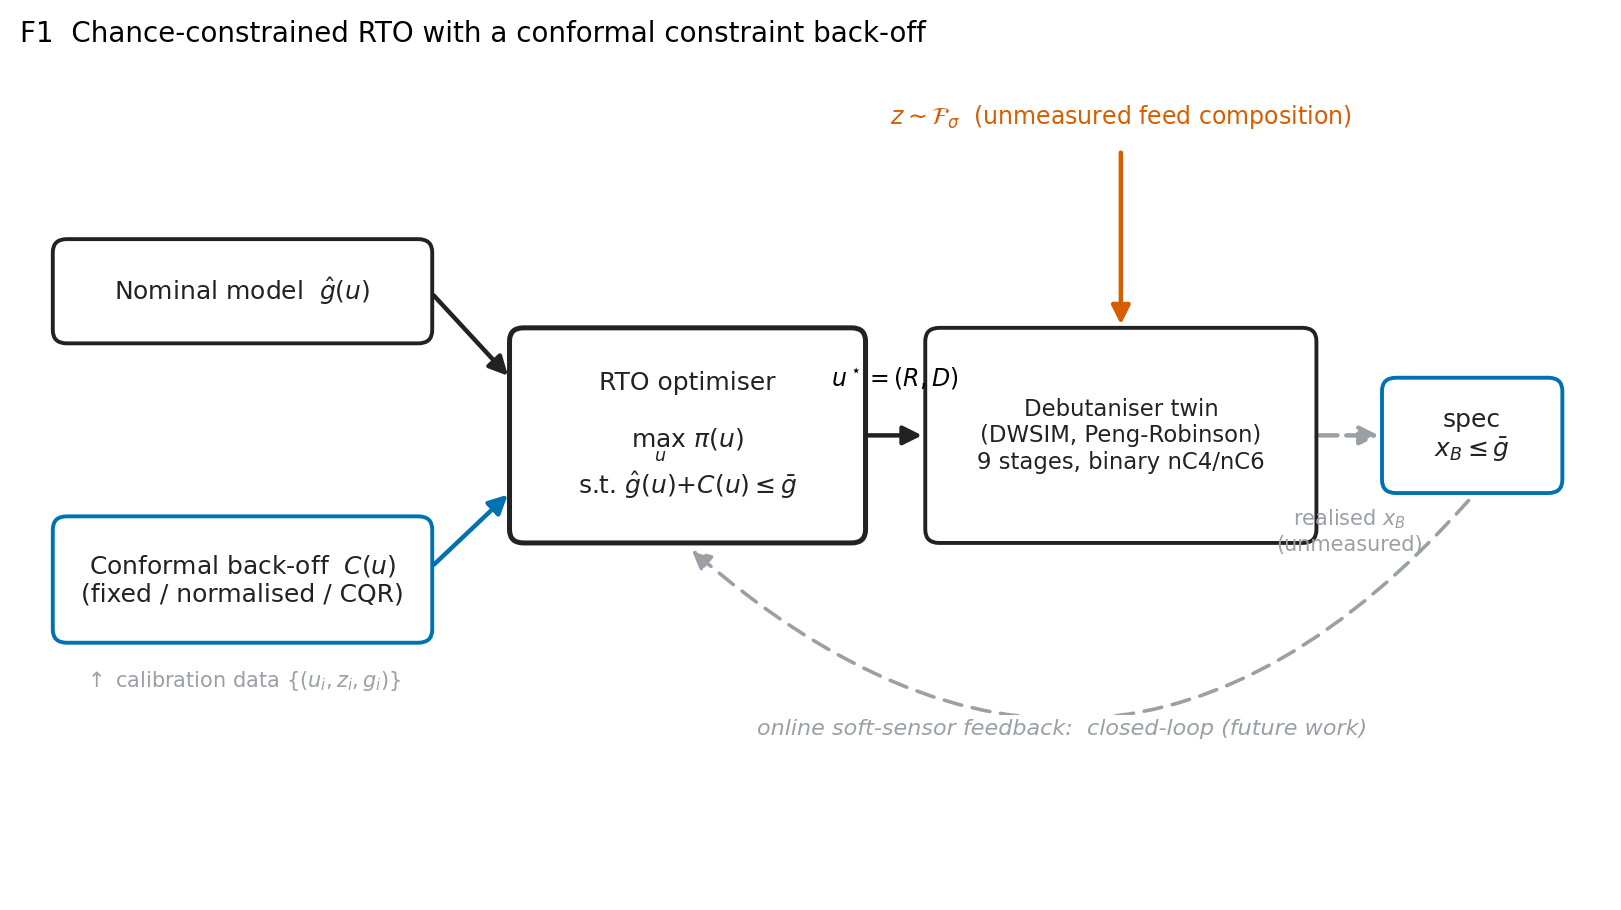
\includegraphics[width=\linewidth]{F1_rto_loop.png}
\caption{Chance-constrained real-time optimisation with a conformal constraint back-off. The
nominal model and the conformal back-off feed the optimiser, which sets the operating point
$(R,D)$ on the twin. The constrained bottoms composition $x_B$ is not measured online; a
closed-loop soft-sensor feedback path (grey, dashed) is left to future work.}
\label{fig:rto}
\end{figure}

\begin{figure}[t]
\centering
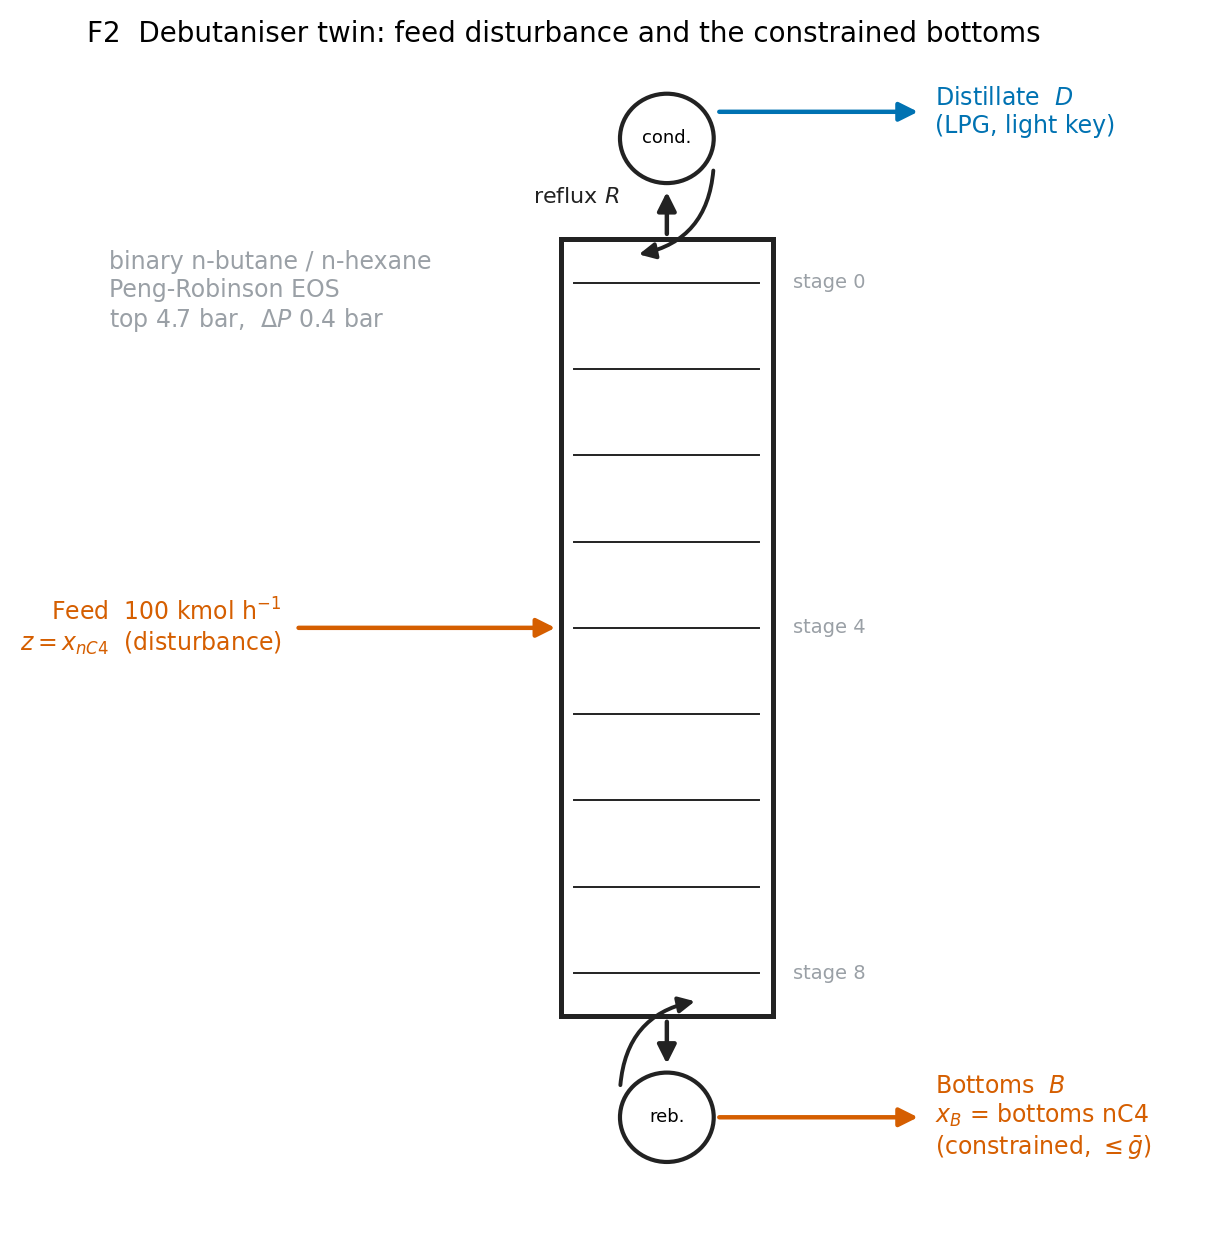
\includegraphics[width=0.72\linewidth]{F2_column.png}
\caption{The debutaniser twin: a nine-stage binary n-butane/n-hexane column under
Peng--Robinson, with the feed-composition disturbance $z$ entering at stage~4, the light-key
distillate overhead, and the constrained bottoms composition $x_B$.}
\label{fig:column}
\end{figure}

\section{Case-study design}
\label{sec:case}

\subsection{Plant evaluations: the feed-composition campaign}

The twin of Section~\ref{sec:methods-twin} is exercised over a grid in the decision and
disturbance variables to produce the plant evaluations all results rest on. The campaign
spans feed light-key fractions $z\in\{0.30,0.325,0.35,0.375,0.40\}$ crossed with reflux
ratios and distillate flows covering the decision box, each case solved to convergence in
DWSIM and screened for mass-balance closure and solver staleness. The accepted set is $77$
operating points. A nominal sub-sweep at $z_0=0.35$ supplies the $15$ points that fit the
optimiser's nominal surfaces $\hat g$, distillate purity, and reboiler duty, while the full
$77$-point set fits the truth surface $g(u,z)$.

Two facts about the campaign shape the design. First, the bottoms composition responds
strongly and monotonically to feed composition: at a fixed mid-box setpoint $x_B$ rises by an
order of magnitude across the sampled $z$ range, which confirms that the disturbance genuinely
propagates to the constrained quantity and that the monotone-$z$ oracle of
Section~\ref{sec:methods-rto} is well founded. Second, the specification is physically
unattainable for large feed excursions. For $z\gtrsim0.38$ the minimum achievable $x_B$ within
the distillate-flow bounds exceeds the spec; at $z=0.40$ the column floor is $x_B\approx0.048$,
well above $\bar g=0.02$, because removing enough light key to meet spec would require a
distillate flow outside the operable range. The whole $[0.30,0.40]$ ensemble is therefore
infeasible for any back-off, which is itself the rationale for a tightly controlled feed: the
operational disturbance must be small, consistent with the realistic $\sigma_z\approx0.006$
anchor used below.

\subsection{Disturbance sweep and calibration}

The disturbance magnitude is swept over
\[
\sigma_z\in\{0.004,\,0.006,\,0.008,\,0.010,\,0.015,\,0.020,\,0.025\},
\]
with $\sigma_z=0.006$ taken as the
operationally realistic centre (a well-controlled upstream feed) and the larger values probing
how each method degrades as the feed becomes more variable. For each $\sigma_z$ the calibration
set of Section~\ref{sec:methods-backoffs} is drawn with size scaled to the disturbance,
$n=\lfloor 1500\cdot\max(1,\sigma_z/0.006)\rfloor$, reflecting that the conditional-quantile
estimate needs more data as the disturbance widens; at the realistic centre $n=1500$. All
draws use a fixed seed so the regime map reproduces exactly on a given platform.

\subsection{Methods compared}

Four back-off constructions enter the comparison. The oracle (the true conditional quantile,
Section~\ref{sec:methods-rto}) is the achievable benchmark. The constant margin
($C_{\mathrm{fix}}$) and the normalised, adaptive back-off ($C_{\mathrm{nrm}}$) are the two
marginally valid baselines, the latter being the soft-sensor-style interval our earlier
design used. The conditional method, CQR with a-posteriori calibration ($C_{\mathrm{cqr}}$
followed by the $\kappa$-step of Section~\ref{sec:methods-apost}), is the proposed remedy.
Each method produces a back-off field over the decision box; the RTO of
Eq.~\eqref{eq:backoff} selects the profit-maximising feasible setpoint; and that setpoint is
then scored against the truth surface.

\subsection{Metrics and protocol}

The primary metric is the realised constraint-violation rate at the selected setpoint, $\hat
v(u^\star)=\widehat{\mathbb P}_z[g(u^\star,z)>\bar g]$, estimated by Monte-Carlo over the
disturbance with $4$ to $6\times10^{3}$ draws; the target is $\hat v\le\alpha=0.10$. The
secondary metric is the operating profit $\pi(u^\star)$, reported only to show that calibrated
safety is not bought at a cost in profit, never as a performance claim in its own right,
because at realistic disturbance the constraint is barely active and all methods sit within a
fraction of a percent of the deterministic optimum. Feasibility is itself an outcome: a method
is reported infeasible at a given $\sigma_z$ when no back-off, after a-posteriori inflation
where applicable, admits a setpoint meeting the target. The a-posteriori inflation factor
$\kappa^\star$ is logged as a diagnostic of data adequacy.

Because the realised violation is a Monte-Carlo quantity, the reported rates carry sampling
noise of order $\pm0.01$ to $0.02$ across platforms even though they are seeded within a
platform; the regime structure and the magnitude of the selection effect are stable to this
noise. The truth surface itself is validated by a leave-one-feed-composition-slice-out test,
fitting on all $z\neq0.375$ and predicting the held-out $z=0.375$ slice, which bounds the
accuracy of every violation estimate (Section~\ref{sec:results-valid}). The specification is
$\bar g=0.02$, the miss level $\alpha=0.10$, the decision box $[0.8,3.0]\times[33,37]$, and the
master seed $20260614$ throughout.

\section{Results}
\label{sec:results}

The four back-off constructions are compared across the disturbance sweep on the committed
twin data (seed $20260614$). Table~\ref{tab:regime} is the full regime map and
Figure~\ref{fig:violation} its headline projection: realised violation against disturbance
magnitude for every method, with the nominal target $\alpha=0.10$ marked. The reading is
consistent across the sweep, and we summarise it method by method below.

\subsection{The selection effect: marginal back-offs are unsafe under optimisation}
\label{sec:results-selection}

The normalised, adaptive back-off, the soft-sensor-style interval that is marginally valid by
construction, fails dramatically. Its realised violation sits between $0.43$ and $0.50$ across
the entire disturbance range against the $0.10$ target, roughly five times the nominal level,
with no dependence on $\sigma_z$. The failure is structural rather than a matter of the
disturbance being large. The mechanism is visible in the selected setpoint
(Figure~\ref{fig:fields}). At every $\sigma_z$ the adaptive method drives the optimiser to the
low-$D$ corner near $R\approx2.83$ and $D\approx33.7$, close to the deterministic optimum,
where the back-off is smallest relative to the true local risk. This is precisely the
operating point the selection-effect argument of Section~\ref{sec:methods-selection} predicts:
among feasible points the optimiser takes the most profitable, which is the one where the
marginally calibrated margin under-covers the conditional quantile. Making the interval
adaptive in width does not help, because the smooth scale model still leaves under-covered
pockets for the optimiser to occupy.

The constant margin is less catastrophic but still unsafe, and ultimately unusable. At small
disturbance it over-violates modestly, between $0.17$ and $0.19$ for $\sigma_z\le0.006$,
because a single margin sized to the pooled residual is too loose where the column is sensitive
and too tight where it is not. For $\sigma_z\ge0.015$ no constant margin admits a feasible
setpoint at all, since the margin required to cover the worst region of the box exceeds the
spec headroom everywhere. Neither marginal construction controls the violation rate that the
chance constraint demands.

\subsection{The oracle confirms the chance constraint is sound}
\label{sec:results-oracle}

That the marginal methods fail is a property of the back-off, not of the formulation. The
oracle back-off, the true conditional quantile, available here because the twin furnishes the
plant response, realises a violation between $0.079$ and $0.106$ across all seven disturbance
levels, that is approximately $\alpha$ by construction, and it remains feasible to the largest
$\sigma_z$ tested. The oracle is not a deployable method, since it needs the plant it is meant
to protect, but it certifies two things. The chance-constrained RTO of Eq.~\eqref{eq:chance} is
correctly posed, and a back-off that is conditionally correct controls the violation rate
exactly where the marginal ones do not. The oracle is therefore the bar the data-driven
conditional method must reach.

\subsection{Conditional calibration restores violation control}
\label{sec:results-fix}

The proposed method, CQR with a-posteriori calibration, tracks the oracle. Its realised
violation is between $0.063$ and $0.105$ for $\sigma_z\le0.020$, within about $0.01$ of the
oracle at every level and inside the target band, and it achieves this at near-oracle profit,
since the CQR and oracle profit columns of Table~\ref{tab:regime} differ by at most a few
dollars per hour at each $\sigma_z$. Two features distinguish it from the marginal baselines.
It selects setpoints that move with the disturbance, from $D\approx34.3$ at the realistic
$\sigma_z=0.006$ out to $D\approx36.6$ at $\sigma_z=0.020$, backing the column away from the
corner as the feed becomes more variable, exactly as the conditional risk requires and exactly
what the marginal methods fail to do. And where the residual finite-sample gap would otherwise
let it violate, the a-posteriori step closes it: at $\sigma_z=0.006$ the conditional quantile
alone is slightly optimistic, and the inflation $\kappa=1.53$ restores the target, with the
reported violation taken on an independent test draw. The conditional construction supplies the
right shape of back-off, and the a-posteriori step supplies the right scale.

\subsection{The boundary: conditional estimation runs out of data}
\label{sec:results-boundary}

The conditional method is not unconditionally safe. It degrades, gracefully and diagnosably, as
the disturbance outgrows the calibration set, and the a-posteriori inflation $\kappa$ is the
signal (Figure~\ref{fig:kappa}). For $\sigma_z\le0.010$ it stays near unity, between $1.0$ and
$1.5$, since the conditional estimate is already close to correct and little stretching is
needed. At $\sigma_z=0.015$ it jumps to $5.78$: the estimate must be stretched nearly sixfold to
be certified safe, and the method is operating at the edge of its feasible-$\kappa$ window. At
$\sigma_z=0.025$, more than four times the realistic disturbance, no feasible inflation certifies
the target and the method is reported infeasible, even though the oracle remains feasible there.
The gap between the two is the finite-sample cost of not knowing the plant. With the truth
surface the conditional quantile is exact; estimated from a calibration set whose support must
widen with $\sigma_z$, it eventually cannot be pinned down tightly enough for an optimiser to
lean on. The $\kappa$ trace makes this a readable property of the method rather than a silent
failure, since the operator sees the safety margin being stretched before it breaks.

\subsection{Safety, not profit}
\label{sec:results-profit}

A deliberate non-result is that the proposed method does not earn more money. At the realistic
disturbance the chance constraint is barely active: every method, including the deterministic
optimum at a profit of about \$5393\,h$^{-1}$, lies within $0.5\%$ of every other
(Table~\ref{tab:regime}; Figure~\ref{fig:profit}). The marginally higher profit of the unsafe
adaptive method is not an advantage. It is the profit of operating at a setpoint that violates
the spec half the time. The contribution is therefore not a profit improvement but calibrated
violation control at no cost in profit: the conditional method buys safety that the marginal
methods cannot deliver, while giving up essentially nothing in operating profit at the realistic
operating point. The profit separation between methods opens up only as $\sigma_z$ grows and the
constraint begins to bind, at which point the marginal methods are already either grossly
violating or infeasible.

\subsection{Surrogate validation and precision accounting}
\label{sec:results-valid}

Every violation rate above is read against the truth surface, so its credibility rests on that
surface interpolating the disturbance faithfully. The leave-one-feed-composition-slice-out test,
fitting on all $z\neq0.375$ and predicting the held-out $z=0.375$ slice, gives $R^2=0.917$ and a
mean absolute error of $0.0053$ in $x_B$ over $15$ held-out points (Figure~\ref{fig:validation}).
That error is the precision floor on the violation estimates. It is why the oracle lands between
$0.08$ and $0.11$ rather than exactly $0.10$, and it bounds how finely any method's violation can
be resolved. Layered on top is the Monte-Carlo sampling noise of the violation estimator itself,
of order $\pm0.01$ to $0.02$ across platforms; re-running the map on a different machine moves
individual rates by at most this much while leaving the regime structure and the fivefold
selection-effect gap intact. We therefore report violation rates as estimates with a band rather
than as point values. The qualitative claims, namely that the marginal back-off fails by about
fivefold, that the conditional method tracks the oracle, and that there is a data-starvation
boundary, all sit far outside that band.

\begin{figure}[t]
\centering
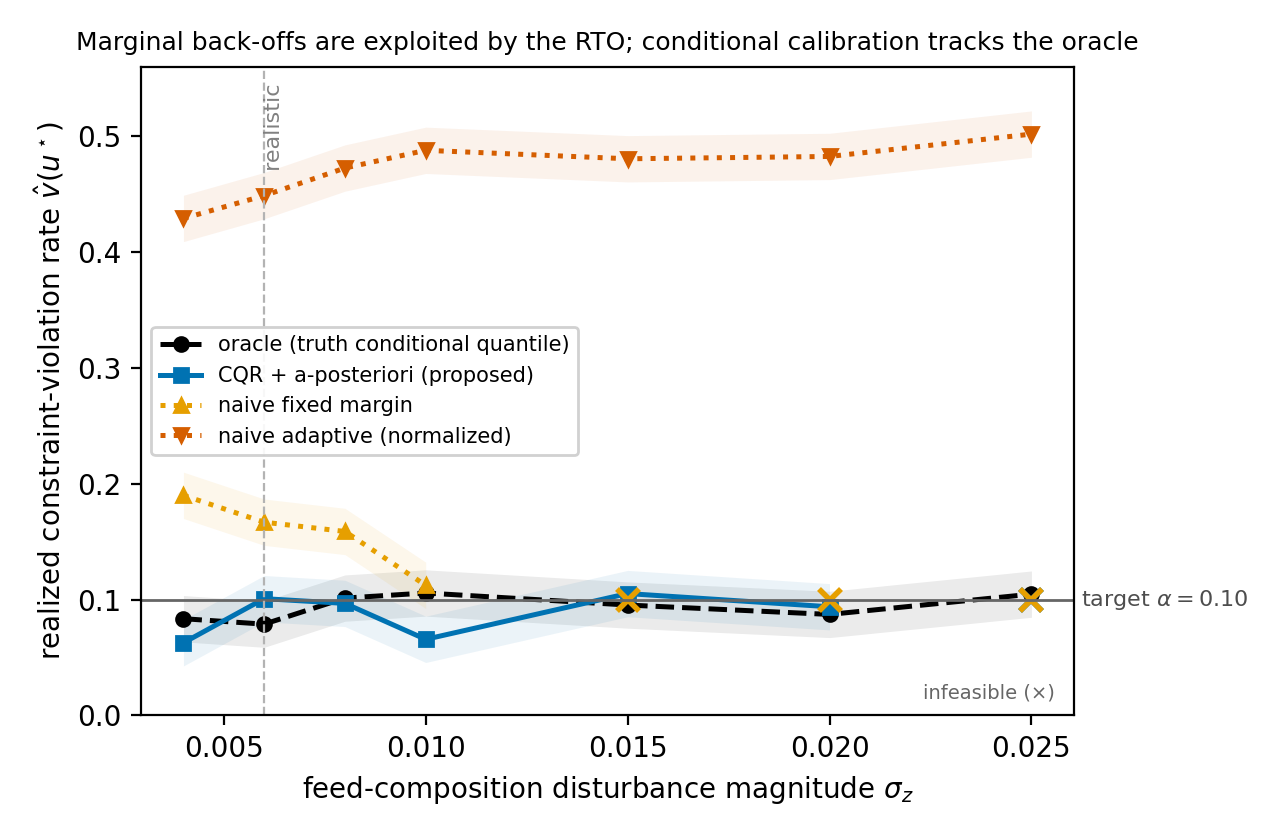
\includegraphics[width=\linewidth]{F3_violation_vs_sigma.png}
\caption{Realised constraint-violation rate versus disturbance magnitude $\sigma_z$ for the four
back-offs, with the nominal target $\alpha=0.10$ and the realistic $\sigma_z$ marked. Crosses
denote infeasible instances; shaded bands are the Monte-Carlo uncertainty. The marginal
back-offs (fixed, normalised) violate well above target, while CQR with a-posteriori calibration
tracks the oracle.}
\label{fig:violation}
\end{figure}

\begin{figure}[t]
\centering
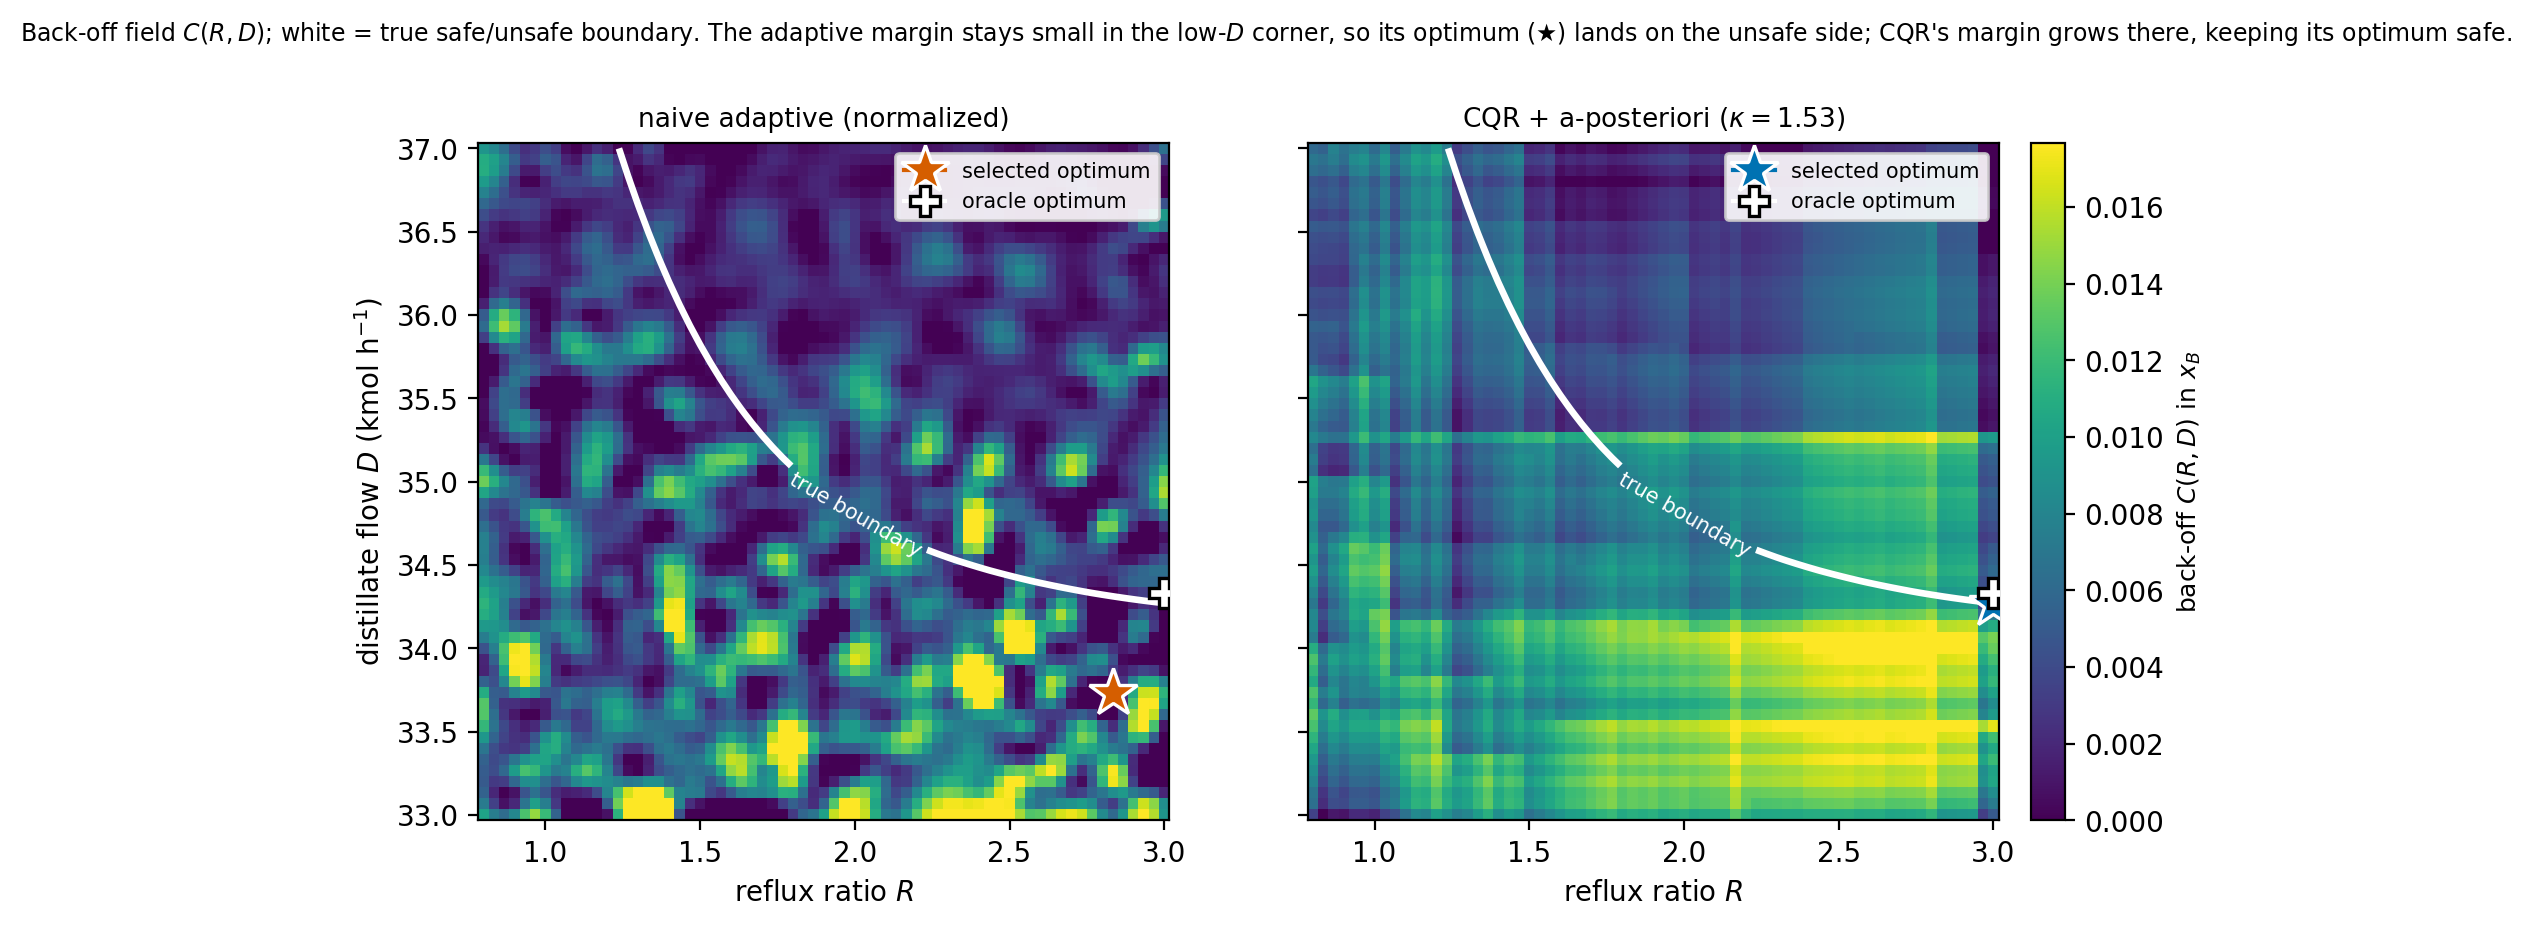
\includegraphics[width=\linewidth]{F4_backoff_fields.png}
\caption{Back-off field $C(R,D)$ at the realistic disturbance for the naive-adaptive and the
CQR+a-posteriori methods, with each method's selected optimum ($\star$) and the oracle optimum.
The white curve is the true feasibility boundary. The adaptive margin stays small in the low-$D$
corner, so its optimum lands on the unsafe side; the CQR margin grows there and keeps its optimum
safe.}
\label{fig:fields}
\end{figure}

\begin{figure}[t]
\centering
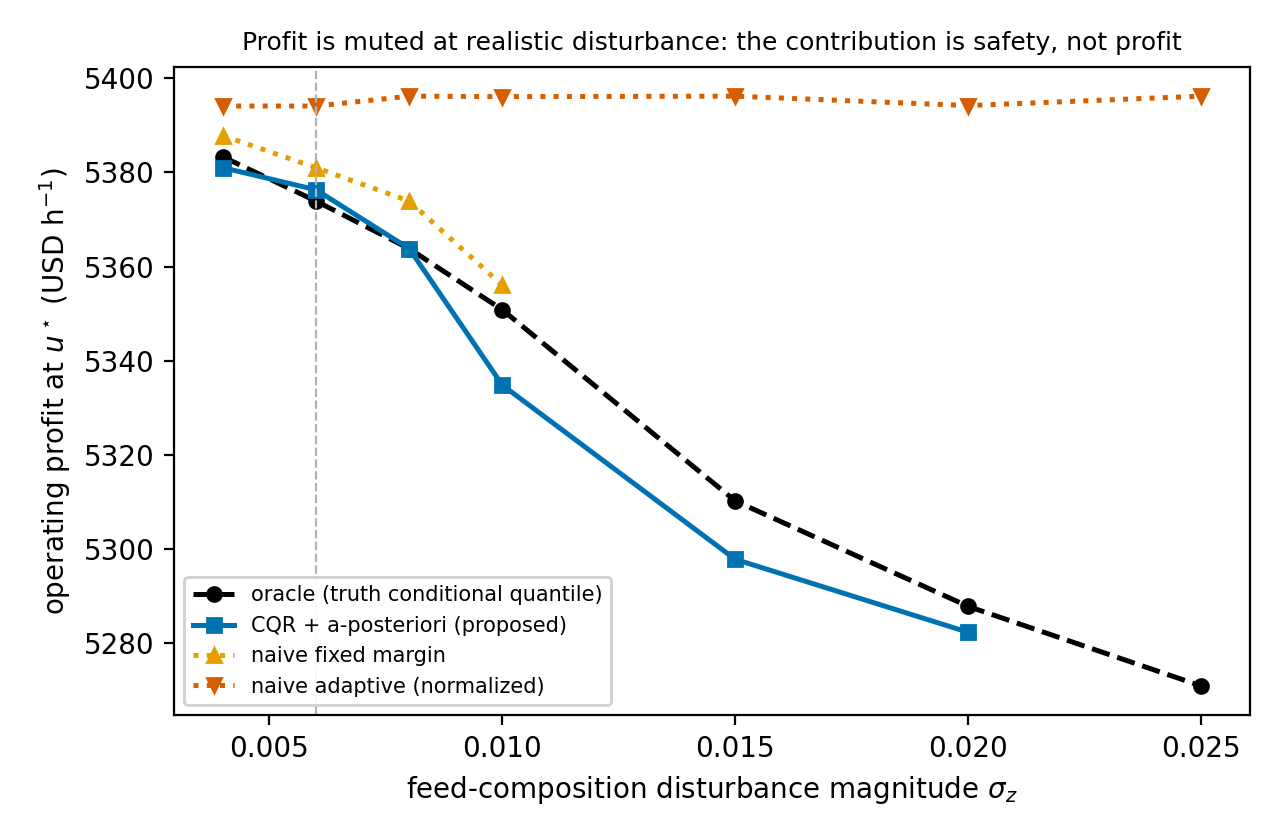
\includegraphics[width=\linewidth]{F5_profit_vs_sigma.png}
\caption{Operating profit at the selected setpoint versus $\sigma_z$. At the realistic
disturbance all methods lie within half a percent of the deterministic optimum; the profit
separation opens only as the constraint begins to bind.}
\label{fig:profit}
\end{figure}

\begin{figure}[t]
\centering
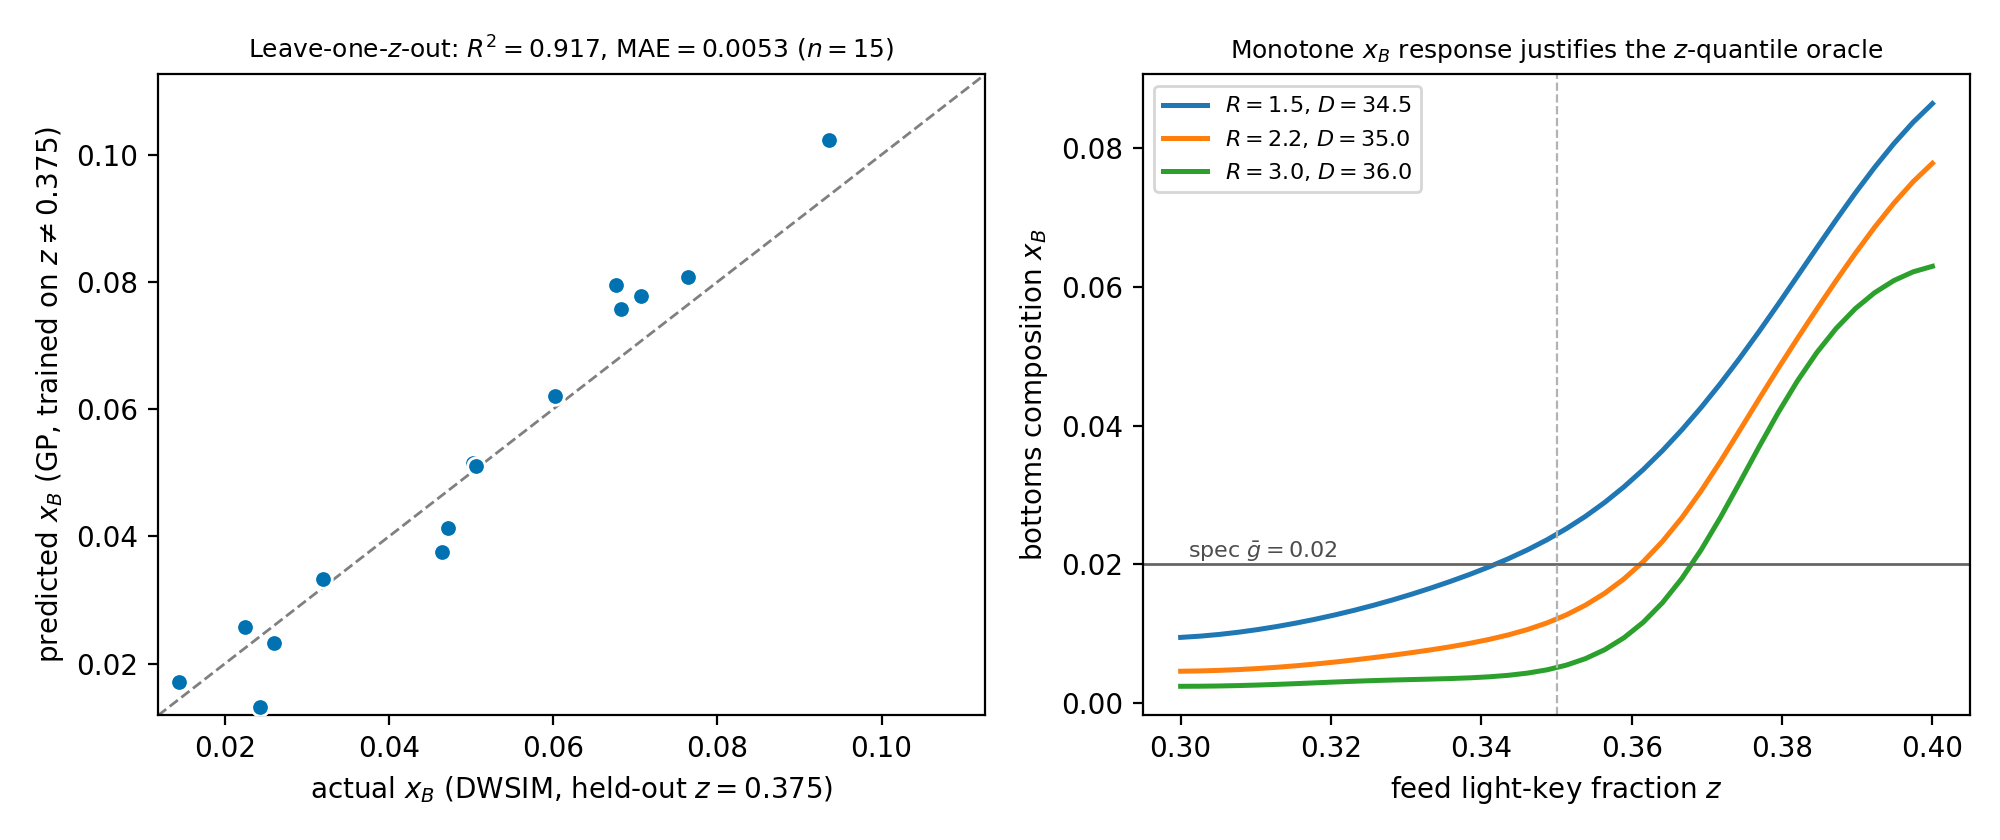
\includegraphics[width=\linewidth]{F6_surrogate_validation.png}
\caption{Truth-surface validation. Left: predicted versus actual $x_B$ on the held-out
$z=0.375$ slice (leave-one-disturbance-out). Right: the monotone $x_B(R,D,z)$ response that
justifies the $z$-quantile oracle.}
\label{fig:validation}
\end{figure}

\begin{figure}[t]
\centering
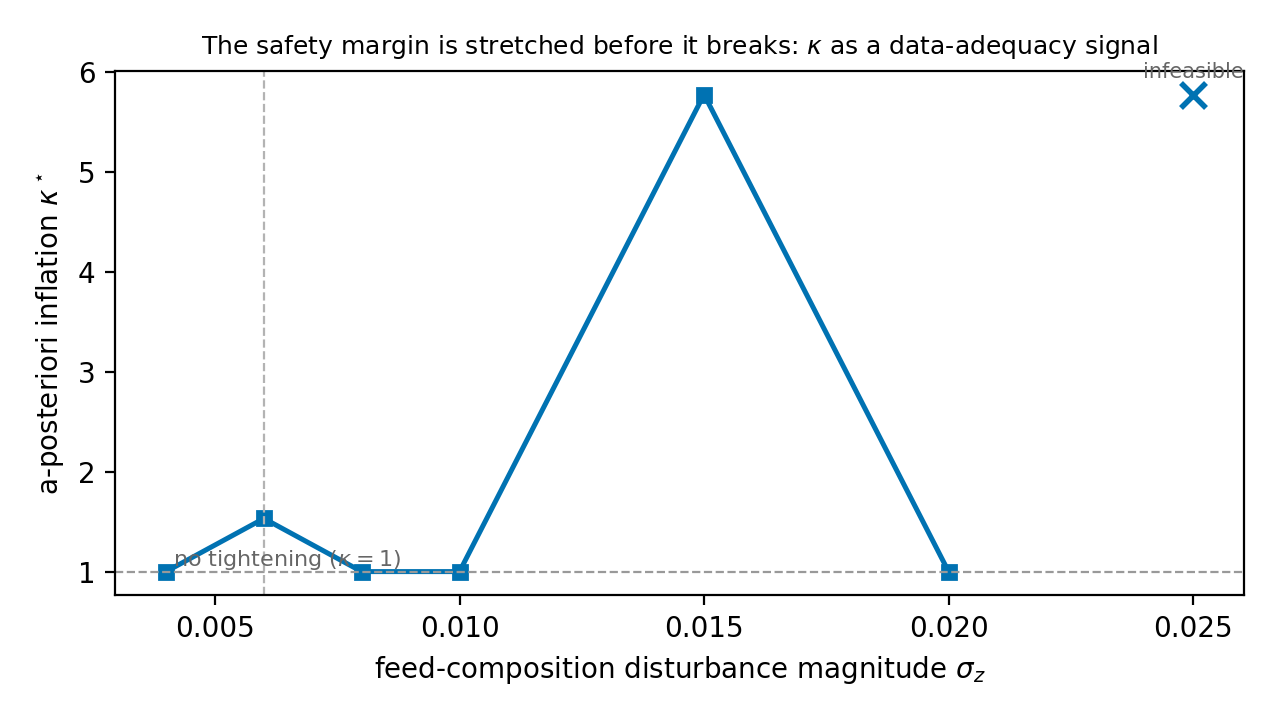
\includegraphics[width=0.8\linewidth]{F7_kappa_vs_sigma.png}
\caption{A-posteriori inflation factor $\kappa^\star$ for the CQR method versus $\sigma_z$. The
margin is stretched (rising $\kappa$) before the method becomes infeasible, making $\kappa^\star$
a readable data-adequacy diagnostic.}
\label{fig:kappa}
\end{figure}

\begin{table}[t]
\centering
\caption{Regime map over disturbance magnitude $\sigma_z$ (canonical run, seed $20260614$,
leave-$z$-out $R^2=0.917$). For each method: operating profit (USD\,h$^{-1}$), realised violation
$\hat v$, a-posteriori inflation $\kappa$, and the selected setpoint $(R^\star,D^\star)$. INF
denotes an infeasible instance. The realistic disturbance is $\sigma_z=0.006$.}
\label{tab:regime}
\footnotesize
\begin{tabular}{llrrrrr}
\toprule
$\sigma_z$ & method & profit & $\hat v$ & $\kappa$ & $R^\star$ & $D^\star$ \\
\midrule
0.004 & oracle      & 5383 & 0.084 & 1.00 & 3.00 & 34.1 \\
      & CQR+apost   & 5381 & 0.063 & 1.00 & 3.00 & 34.1 \\
      & naive-fixed & 5388 & 0.190 & 1.00 & 3.00 & 33.9 \\
      & naive-adapt & 5394 & 0.429 & 1.00 & 2.83 & 33.7 \\
\midrule
0.006 & oracle      & 5374 & 0.079 & 1.00 & 3.00 & 34.3 \\
      & CQR+apost   & 5376 & 0.101 & 1.53 & 3.00 & 34.3 \\
      & naive-fixed & 5381 & 0.167 & 1.00 & 3.00 & 34.1 \\
      & naive-adapt & 5394 & 0.449 & 1.00 & 2.83 & 33.7 \\
\midrule
0.008 & oracle      & 5364 & 0.101 & 1.00 & 2.83 & 34.6 \\
      & CQR+apost   & 5364 & 0.097 & 1.00 & 2.83 & 34.6 \\
      & naive-fixed & 5374 & 0.159 & 1.00 & 3.00 & 34.3 \\
      & naive-adapt & 5396 & 0.472 & 1.00 & 3.00 & 33.7 \\
\midrule
0.010 & oracle      & 5351 & 0.106 & 1.00 & 2.80 & 34.9 \\
      & CQR+apost   & 5335 & 0.066 & 1.00 & 2.60 & 35.3 \\
      & naive-fixed & 5356 & 0.112 & 1.00 & 2.93 & 34.8 \\
      & naive-adapt & 5396 & 0.488 & 1.00 & 2.93 & 33.7 \\
\midrule
0.015 & oracle      & 5310 & 0.095 & 1.00 & 2.43 & 35.9 \\
      & CQR+apost   & 5298 & 0.105 & 5.78 & 3.00 & 36.2 \\
      & naive-fixed & \multicolumn{5}{c}{INF} \\
      & naive-adapt & 5396 & 0.480 & 1.00 & 3.00 & 33.7 \\
\midrule
0.020 & oracle      & 5288 & 0.087 & 1.00 & 2.20 & 36.5 \\
      & CQR+apost   & 5282 & 0.094 & 1.00 & 2.37 & 36.6 \\
      & naive-fixed & \multicolumn{5}{c}{INF} \\
      & naive-adapt & 5394 & 0.482 & 1.00 & 3.00 & 33.7 \\
\midrule
0.025 & oracle      & 5271 & 0.105 & 1.00 & 2.23 & 36.9 \\
      & CQR+apost   & \multicolumn{5}{c}{INF} \\
      & naive-fixed & \multicolumn{5}{c}{INF} \\
      & naive-adapt & 5396 & 0.502 & 1.00 & 3.00 & 33.7 \\
\bottomrule
\end{tabular}
\end{table}

\section{Discussion}
\label{sec:discussion}

\subsection{The general lesson: conformal-in-the-loop needs conditional validity}

The result is narrow in its case study but general in its mechanism. Nothing in the
selection-effect argument of Section~\ref{sec:methods-selection} is specific to a debutaniser or
to feed composition. It follows from two facts that hold whenever a conformal interval is placed
inside an optimisation. First, split and locally adaptive conformal prediction guarantee
coverage marginally, averaged over the calibration distribution, and the conditional coverage
varies across the input space. Second, an optimiser is a selection operator that seeks the
boundary of the feasible region and therefore lands preferentially where the margin is tightest
relative to the local risk, which is where coverage is worst. Any pipeline with these two
features, a marginally calibrated margin and an optimiser pressing on it, will show the same
degradation. This includes back-offs in stochastic and learning-based model-predictive control,
constraint handling in safe Bayesian optimisation, and any chance-constrained program that sizes
its margin from a marginally valid predictor. The practical implication is a design rule: a
conformal margin used as a hard optimisation constraint must be conditionally valid at the
operating point, not merely marginally valid over a calibration set. Where conditional validity
cannot be guaranteed in advance, an a-posteriori calibration at the selected solution
\citep{zhao2024cpp} is necessary, but, as Section~\ref{sec:results-boundary} shows, that step is
small and reliable only when the base margin is already conditional. On a marginal base it must
inflate the margin severalfold, and it can fail outright.

\subsection{What the method does and does not buy}

The contribution is calibrated violation control, and the honest accounting of its value has two
parts. On safety, the conditional method delivers what the marginal baselines cannot, a realised
violation that tracks the oracle to within the Monte-Carlo band across the operationally
realistic disturbance range, where the naive-adaptive margin violates roughly five times the
nominal rate and the fixed margin is either over-violating or infeasible. On profit, the method
buys essentially nothing at the realistic operating point, where every method, including the
deterministic optimum, lies within half a percent, because at a well-controlled feed the chance
constraint is barely active. We regard the second fact as a feature of the honest framing rather
than a weakness. The value of a safety margin is not that it raises profit but that it removes a
violation the unsafe alternative incurs while appearing to be slightly more profitable. The
profit separation widens only as the disturbance grows and the constraint begins to bind, by
which point the marginal methods have already failed. A reader looking for a profit headline will
not find one here, and should not, because the result is about constraint integrity under
uncertainty.

\subsection{Limitations}

Several boundaries should be read with the result. The plant is a simulation twin, a rigorous
DWSIM Peng--Robinson model validated by leave-one-disturbance-out interpolation ($R^2=0.917$, MAE
$0.0053$ in $x_B$), but it is not plant data; the selection-effect mechanism is structural and
should transfer, yet the specific magnitudes, the fivefold factor and the regime boundaries, are
twin-specific. The study uses a single binary n-butane and n-hexane system, one unmeasured
disturbance (feed composition), and a two-dimensional decision. A higher-dimensional decision or
several simultaneous disturbances would enlarge the space over which the conditional quantile must
be estimated, and would therefore bring the data-starvation boundary of
Section~\ref{sec:results-boundary} to smaller disturbance magnitudes than observed here. The
reported violation rates are Monte-Carlo estimates carrying a band of $\pm0.01$ to $0.02$, and the
truth-surface error, about $0.005$ in $x_B$, is a precision floor below which no violation
difference can be resolved; the qualitative claims sit far outside that band, but fine rankings
near the target should not be over-read. The oracle is a benchmark, not a method, because it uses
the true plant response and the monotone-in-$z$ structure to evaluate the conditional quantile in
one shot; the conformal methods make no monotonicity assumption, but a non-monotone or multi-modal
constraint response would require the oracle itself to be estimated rather than read off, which
complicates only the benchmark and not the proposed method. Finally, the a-posteriori step
requires an independent calibration draw at the selected setpoint; in deployment this is a
held-out window of operating data, and its size sets how tightly the residual gap can be closed.

\subsection{Toward closed-loop and plant deployment}

This paper is the static, open-loop foundation, in which the disturbance is unmeasured and the
optimiser commits to a setpoint under a calibrated margin. The natural extension is closed-loop,
where an online estimate of the constrained quantity, supplied by the soft sensor of the companion
paper that infers the unmeasured composition from tray temperatures, feeds back so that the
back-off contracts as the disturbance becomes partially observed and the operating point tracks
it. That closed-loop study, with the sensor in the loop and the disturbance evolving in time, is
left to future work, and the exchangeability questions it raises, calibration under feedback and
temporal dependence, connect directly to the beyond-exchangeability conformal literature of
Section~\ref{sec:related}. The other clear next steps are validation on plant or pilot data, where
the disturbance law is empirical rather than assumed, and extension to multi-component products
and higher-dimensional decisions, where the cost of conditional estimation is the binding
constraint. In all of these, the design rule above is the portable result: size the margin
conditionally, and read the a-posteriori inflation as the signal that the data can no longer
certify the target.

\section{Conclusion}
\label{sec:conclusion}

Real-time optimisation must subtract a back-off from a quality specification to protect a
constraint it cannot measure, and conformal prediction is the natural distribution-free way to
size that back-off. We have shown that the natural choice is unsafe. An optimiser pressing on a
marginally valid conformal margin, even a locally adaptive one, behaves as a selection mechanism
that drives the operating point to where the margin under-covers the conditional constraint
quantile, so the realised violation reaches roughly five times the nominal level across the
disturbance range. An oracle margin built from the true conditional quantile holds the violation
at the target, which confirms that the failure is in the back-off, not in the chance-constrained
formulation. The remedy is conditional validity. A conformalised-quantile-regression back-off,
with an a-posteriori calibration step at the selected setpoint, returns the realised violation to
the oracle level at near-oracle profit over the operationally realistic disturbance range, and it
degrades only, and diagnosably through a climbing inflation factor, when the disturbance widens
beyond several times the realistic level and the conditional estimate runs out of calibration
data. A regime map over disturbance magnitude characterises where each margin controls violation,
where a constant margin becomes infeasible, and where even the conditional method can no longer
certify the target.

The contribution is calibrated safety, not profit. At a well-controlled feed the constraint is
barely active and all methods earn within half a percent of the deterministic optimum, so the
value of the conditional method is the violation it removes, not the profit it adds. The mechanism
is general, since any conformal interval used as a hard optimisation constraint is exposed to the
same selection effect, and the portable design rule is to size the margin conditionally and to
read the a-posteriori inflation as a signal of data adequacy. Demonstrated here on a rigorous
binary-distillation twin, the approach sets up a closed-loop extension in which an online soft
sensor of the unmeasured quality feeds the back-off as the disturbance is partially observed.

\section*{Reproducibility}
The twin data, the chance-constrained RTO implementation, the regime-map script, and the figure
scripts are in the project repository; the regime map and all figures regenerate from a single
fixed seed.

\bibliographystyle{elsarticle-harv}
\bibliography{references}

\end{document}
